\section{Symbolic Schr\"odinger Equation}
Let \( \psi: \mathbb{Z}_{m} \to \mathbb{R} \) be a discrete wavefunction. The Hamiltonian is:
\[
(H\psi)(x) = -t(\psi(x+1) + \psi(x-1) - 2\psi(x)) + V(x)\psi(x),
\]
with periodic boundary conditions, where \( t = \frac{\hbar^2}{2m} = 0.1 \) (\(\hbar = 1\), \(m = 5\)). Solving \( H\psi = E\psi \), we obtain eigenfunctions \( \psi_k \) and eigenvalues \( E_k \). The ground state \( \psi_0 \) (lowest \( E_0 \)) informs:
\[
V_{\text{mod}}(x) = E_0 - |\psi_0(x)|^2,
\]
where \( \sum_x |\psi_0(x)|^2 = 1 \). The term \( |\psi_0(x)|^2 \) reflects probability density, adjusting \( V_{\text{mod}} \) to emphasize prime-rich classes, indirectly influencing the spectrum toward zeta zeros.

\begin{figure}[t]
\centering
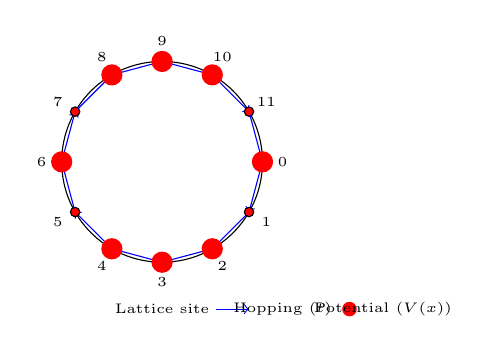
\begin{tikzpicture}[scale=0.85]
    % Schrodinger discretization on a ring
    % Draw a circle for the periodic boundary
    \draw (0,0) circle (1.5);
    
    % Draw the lattice points
    \foreach \i in {0,...,11} {
        \pgfmathsetmacro{\angle}{-\i*30} % 12 points, 360/12 = 30 degrees
        \filldraw (\angle:1.5) circle (2pt);
        
        % Label the points
        \node at (\angle:1.8) {\tiny $\i$};
        
        % Draw the coupling between adjacent points
        \pgfmathsetmacro{\nextangle}{-(\i+1)*30}
        \draw[blue, ->] (\angle:1.5) -- (\nextangle:1.5);
    }
    
    % Draw the potential on-site (as inner dots of varying sizes)
    \foreach \i/\v in {0/1.5, 1/0.5, 2/1.5, 3/1.5, 4/1.5, 5/0.5, 6/1.5, 7/0.5, 8/1.5, 9/1.5, 10/1.5, 11/0.5} {
        \pgfmathsetmacro{\angle}{-\i*30}
        \pgfmathsetmacro{\radius}{0.1*\v}
        \filldraw[red] (\angle:1.5) circle (\radius);
    }
    
    % Add a legend
    \node at (0,-2.2) {\tiny Lattice site};
    \draw[blue, ->] (0.8,-2.2) -- (1.3,-2.2);
    \node at (1.8,-2.2) {\tiny Hopping ($t$)};
    \filldraw[red] (2.8,-2.2) circle (0.1);
    \node at (3.3,-2.2) {\tiny Potential ($V(x)$)};
\end{tikzpicture}
\caption{Discrete Schrödinger equation on a ring of 12 sites, with hopping term $t$ and on-site potential $V(x)$. The size of the red dots represents the potential strength.}
\label{fig:schrodinger_ring}
\end{figure}

% NEW ILLUSTRATION FOR GROUND STATE VISUALIZATION
\begin{figure}[t]
\centering
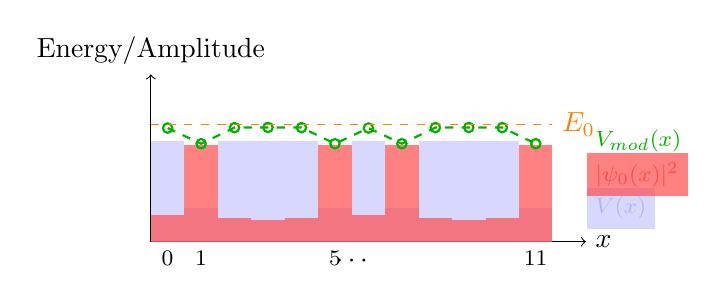
\begin{tikzpicture}[scale=0.85]
    % Setup the axes
    \draw[->] (0,0) -- (6.5,0) node[right] {$x \modm$};
    \draw[->] (0,0) -- (0,2.5) node[above] {Energy/Amplitude};
    
    % Draw the initial potential V(x)
    \foreach \x in {0, 2, 3, 4, 6, 8, 9, 10} {
        \fill[blue!30, opacity=0.5] (0.5*\x, 0) rectangle (0.5*\x + 0.5, 1.5);
    }
    \foreach \x in {1, 5, 7, 11} {
        \fill[blue!30, opacity=0.5] (0.5*\x, 0) rectangle (0.5*\x + 0.5, 0.5);
    }
    
    % Draw the ground state wavefunction amplitude |ψ₀(x)|²
    \foreach \x/\v in {0/0.05, 1/0.18, 2/0.045, 3/0.04, 4/0.045, 5/0.18, 6/0.05, 7/0.18, 8/0.045, 9/0.04, 10/0.045, 11/0.18} {
        \fill[red!70, opacity=0.7] (0.5*\x, 0) rectangle (0.5*\x + 0.5, \v*8);
    }
    
    % Draw the modified potential V_mod(x)
    \foreach \x/\v in {0/1.697506, 1/1.463694, 2/1.704297, 3/1.706590, 4/1.704297, 5/1.463694, 6/1.697506, 7/1.463694, 8/1.704297, 9/1.706590, 10/1.704297, 11/1.463694} {
        \draw[green!70!black, thick] (0.5*\x + 0.25, \v) circle (2pt);
    }
    \draw[green!70!black, thick, dashed] plot coordinates {
        (0.25, 1.697506) (0.75, 1.463694) (1.25, 1.704297) (1.75, 1.706590) 
        (2.25, 1.704297) (2.75, 1.463694) (3.25, 1.697506) (3.75, 1.463694)
        (4.25, 1.704297) (4.75, 1.706590) (5.25, 1.704297) (5.75, 1.463694)
    };
    
    % Add eigenvalue E₀
    \draw[orange, dashed] (0,1.75) -- (6,1.75);
    \node[orange, right] at (6,1.75) {$E_0$};
    
    % Add labels for x-axis
    \foreach \x/\label in {0/0, 1/1, 5/5, 11/11} {
        \node[below] at (0.5*\x + 0.25, 0) {\footnotesize \label};
    }
    \node at (3, -0.3) {$\cdots$};
    
    % Add a legend
    \node[blue!30, fill=blue!30, opacity=0.5, text opacity=1, right] at (6.5,0.5) {\footnotesize $V(x)$};
    \node[red!70, fill=red!70, opacity=0.7, text opacity=1, right] at (6.5,1.0) {\footnotesize $|\psi_0(x)|^2$};
    \node[green!70!black, right] at (6.5,1.5) {\footnotesize $V_{\text{mod}}(x)$};
\end{tikzpicture}
\caption{The ground state solution of the Schrödinger equation: Initial potential $V(x)$ (blue), ground state probability density $|\psi_0(x)|^2$ (red), ground state energy $E_0$ (orange dashed line), and the resulting modified potential $V_{\text{mod}}(x) = E_0 - |\psi_0(x)|^2$ (green). Note how the modified potential enhances prime-rich classes.}
\label{fig:ground_state_solution}
\end{figure}